\documentclass[aspectratio=169]{beamer}

\usepackage[utf8]{inputenc}
\usepackage[spanish]{babel}
\usepackage{graphicx}
\usepackage{booktabs}
\usepackage{ragged2e}
\usepackage{minted}
\usepackage{xcolor}
\usepackage{tikz}
\usepackage{algorithm}
\usepackage{algorithmic}
\usepackage{minted}
\usepackage{listings}
\usepackage{tikz}
\usetikzlibrary{arrows.meta,positioning,fit,shapes.symbols}
\usetikzlibrary{arrows,shapes}
\definecolor{LightGray}{gray}{0.975}
\definecolor{links}{HTML}{2A1B81}
\hypersetup{colorlinks,linkcolor=,urlcolor=blue}
\AtBeginEnvironment{minted}{%
  \renewcommand{\fcolorbox}[4][]{#4}}

\usefonttheme{serif}

\usepackage{listings}
\lstdefinestyle{myCustomSQLStyle}{
  language=SQL,
  numbers=left,
  stepnumber=1,
  numbersep=10pt,
  tabsize=4,
  frame=single,
  backgroundcolor=\color{LightGray},
  breaklines=true,
  showspaces=false,
  showstringspaces=false
}

\newcommand\Wider[2][18mm]{%
    \makebox[\linewidth][c]{%
        \begin{minipage}{\dimexpr\textwidth+#1\relax}
            \raggedright#2
        \end{minipage}%
    }%
}

\title[SVM]{Emergent Digital Technologies}
\subtitle{Support Vector Machines (SVM)}
\author{Brad Boehmke \& Brandon Greenwell}
\date{\today}

% Remove navigation symbols...
\setbeamertemplate{navigation symbols}{}

\defbeamertemplate*{footline}{shadow theme}{
    \leavevmode
    \hbox{
        \begin{beamercolorbox}[
                wd =        0.33\paperwidth,
                ht =        2.5ex,
                dp =        1.125ex,
                leftskip =  0.3cm plus1fil,
                rightskip = 0.3cm
            ]{author in head/foot}
            \flushleft EDT
        \end{beamercolorbox}
        \begin{beamercolorbox}[
                wd =        0.33\paperwidth,
                ht =        2.5ex,
                dp =        1.125ex,
                leftskip =  0.3cm plus1fil,
                rightskip = 0.3cm
            ]{author in head/foot}
            \insertshorttitle
        \end{beamercolorbox}
        \begin{beamercolorbox}[
                wd =        0.33\paperwidth,
                ht =        2.5ex,
                dp =        1.125ex,
                leftskip =  0.3cm plus1fil,
                rightskip = 0.3cm
            ]{title in head/foot}
            \hfill \insertframenumber\,/\,\inserttotalframenumber%
        \end{beamercolorbox}
    }
}

\AtBeginSection[]{
    \begin{frame}<beamer>
        \frametitle{Plan}
        \tableofcontents[currentsection]
    \end{frame}
}

\newcommand{\toRight}[1]{
    \begin{FlushRight}
        {\tiny #1}
    \end{FlushRight}
}

\begin{document}

\frame{\titlepage}

\begin{frame}{Hands-On Machine Learning with R}
    \vspace{1mm}
    \centering
    
\includegraphics[height=0.75\textheight]{figures/book_cover.jpg} \\
    \vspace{1mm}
    {
        \scriptsize
        Content has been extracted from \textit{Hands-On Machine Learning with R}, by Boehmke, B. \& Greenwell, B. CRC Press. 2019.
        Visit \url{https://bradleyboehmke.github.io/HOML/}.
    }
\end{frame}

\begin{frame}{Introduction to Support Vector Machines}
    \begin{itemize}
        \item SVMs offer a direct approach to binary classification.
        \item The goal is to find a \textbf{hyperplane} in a feature space that ``best'' separates two classes.
        \item Two main extensions make SVMs powerful in practice:
        \begin{enumerate}
            \item Loosening the requirement for ``perfect'' separation.
            \item Using the \textbf{kernel trick} to enlarge the feature space for better separation.
        \end{enumerate}
    \end{itemize}
\end{frame}

\begin{frame}{R Implementation Prerequisites}
    \begin{itemize}
        \item Key packages for SVM in R:
        \begin{itemize}
            \item \texttt{kernlab}: The most flexible implementation for fitting SVMs.
            \item \texttt{caret}: Used for tuning hyperparameters and pre-processing.
            \item \texttt{e1071}: An alternative package for SVM implementation.
        \end{itemize}
        \item Interpretability tools:
        \begin{itemize}
            \item \texttt{vip}: For variable importance plots.
            \item \texttt{pdp}: For partial dependence plots.
        \end{itemize}
    \end{itemize}
\end{frame}

\begin{frame}{Optimal Separating Hyperplanes}
    \begin{itemize}
        \item A hyperplane in $p$-dimensional space is defined by:

        $$f(X) = \beta_0 + \beta_1 X_1 + \dots + \beta_p X_p = 0$$

        \item For $p=2$, it's a line; for $p=3$, it's a plane.
        \item The hyperplane acts as a \textbf{decision boundary}.
        \item Points are classified based on which side of the boundary they fall ($f(X) > 0$ or $f(X) < 0$).
    \end{itemize}
\end{frame}

\begin{frame}{Optimal Separating Hyperplanes (Cont.)}
    \centering
    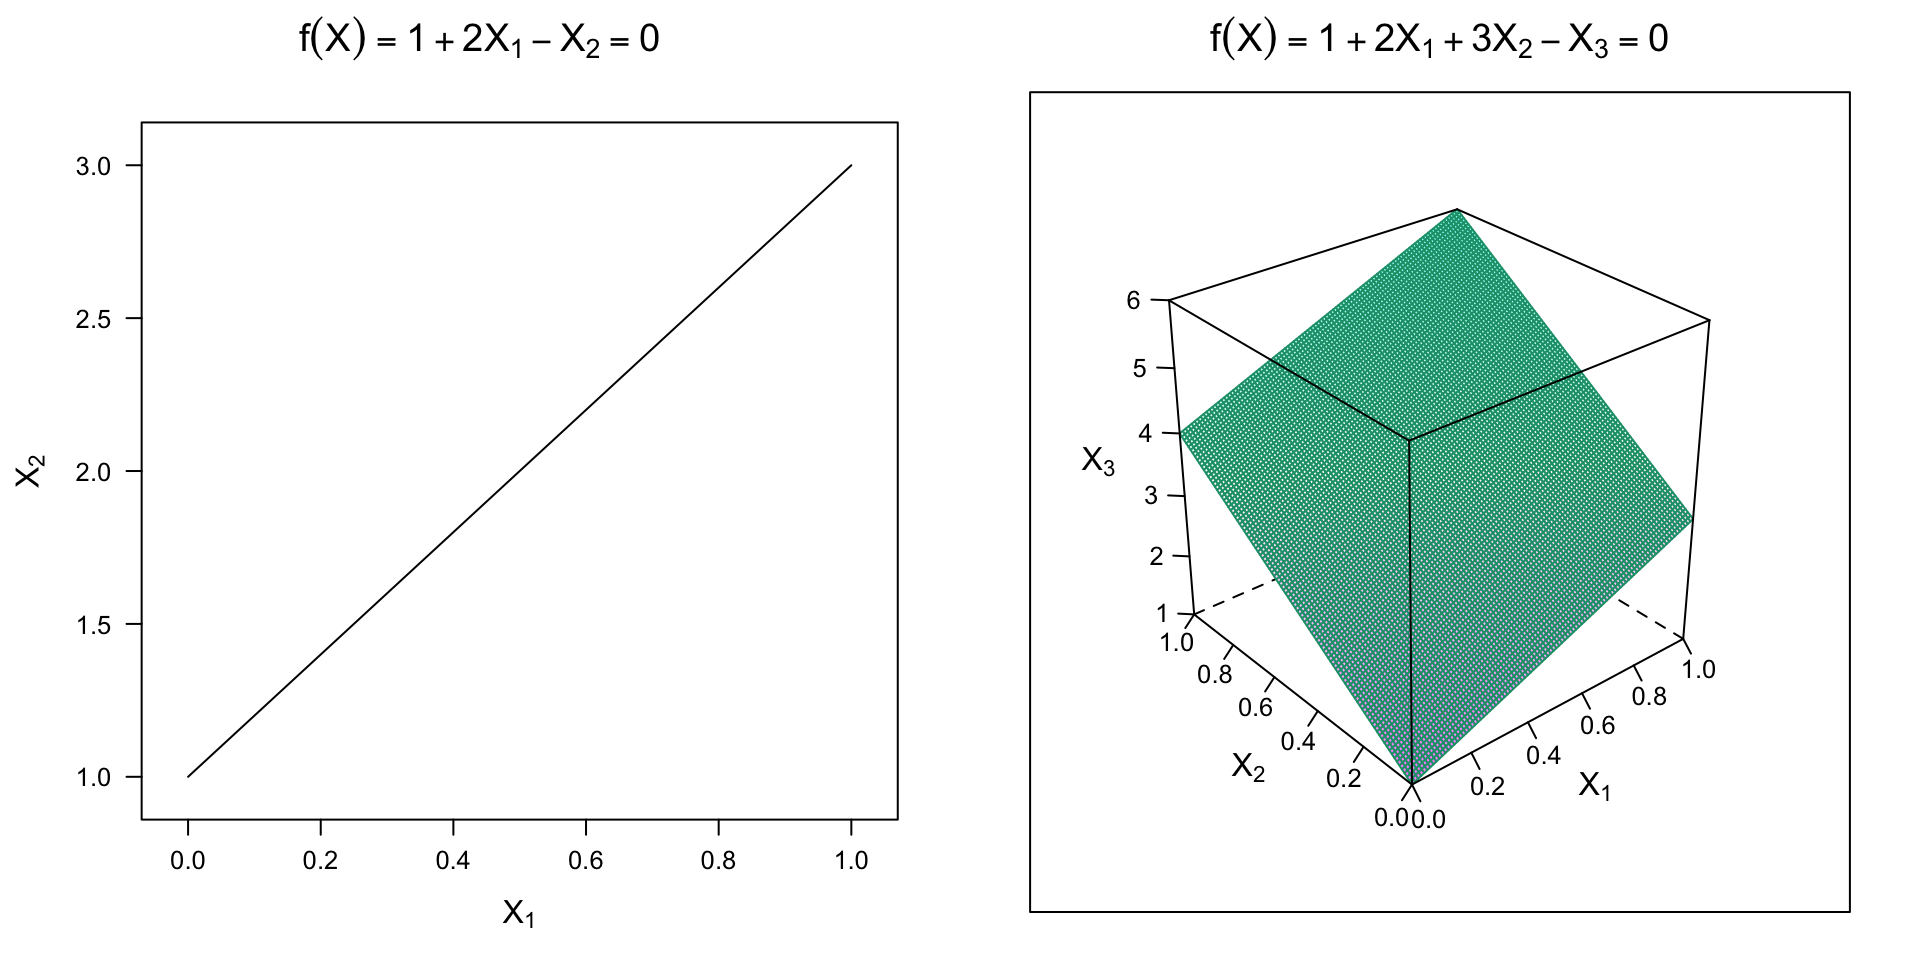
\includegraphics[width=0.9\textwidth]{figures/hyperplanes_1}
\end{frame}

\begin{frame}{Optimal Separating Hyperplanes (Cont.)}
    \centering
    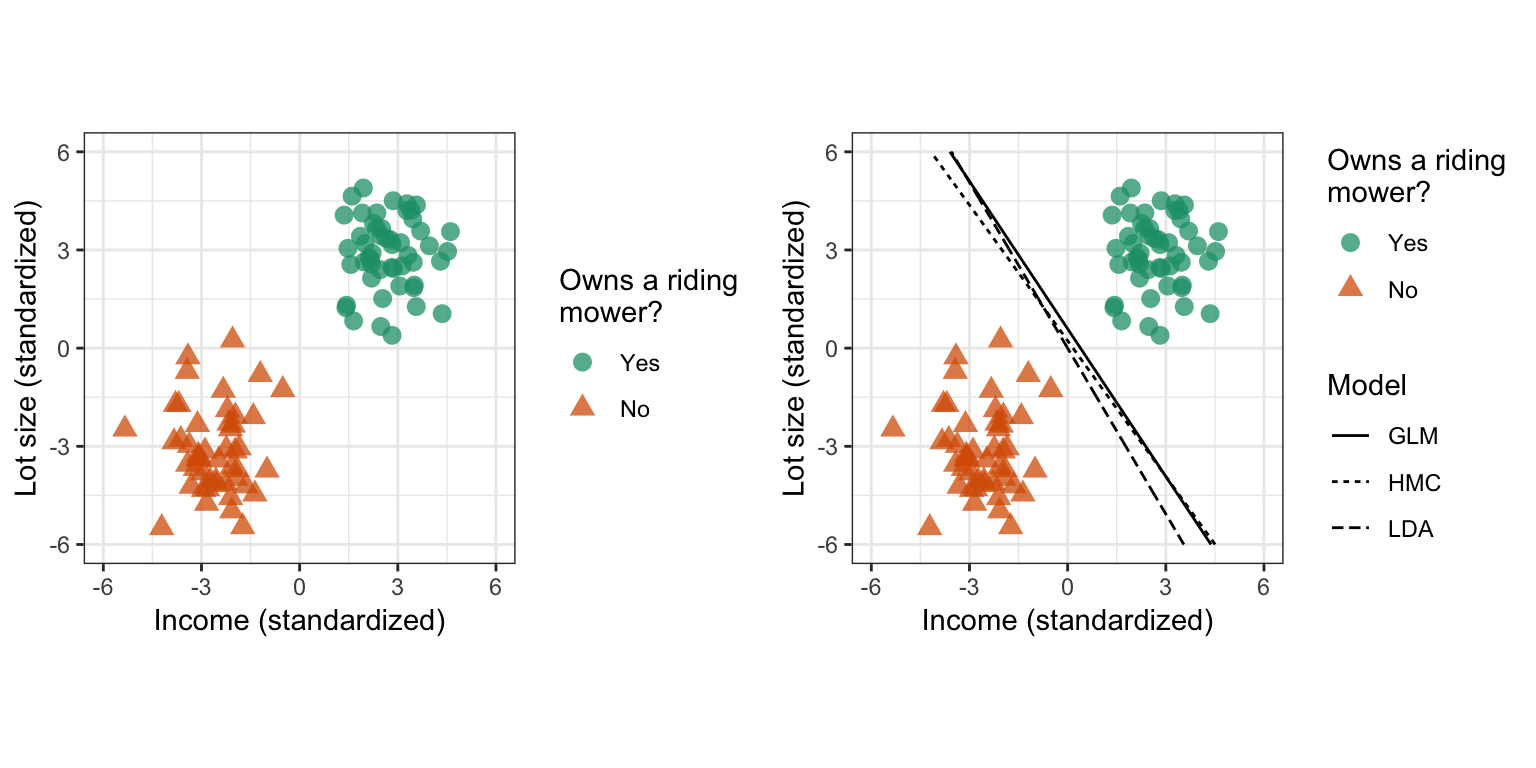
\includegraphics[width=0.9\textwidth]{figures/hyperplanes_2}
\end{frame}

\begin{frame}{The Hard Margin Classifier (HMC)}
    \begin{itemize}
        \item If classes are perfectly separable, HMC finds the boundary that provides \textbf{maximum separation}.
        \item It maximizes the distance to the closest points from either class.
        \item This distance is called the \textbf{margin (M)}.
        \item Geometric construction:
        \begin{enumerate}
            \item Draw convex hulls around each class.
            \item Find the shortest line segment connecting the hulls.
            \item The perpendicular bisector of this segment is the HMC.
        \end{enumerate}
    \end{itemize}
\end{frame}

\begin{frame}{The Hard Margin Classifier (Cont.)}
    \centering
    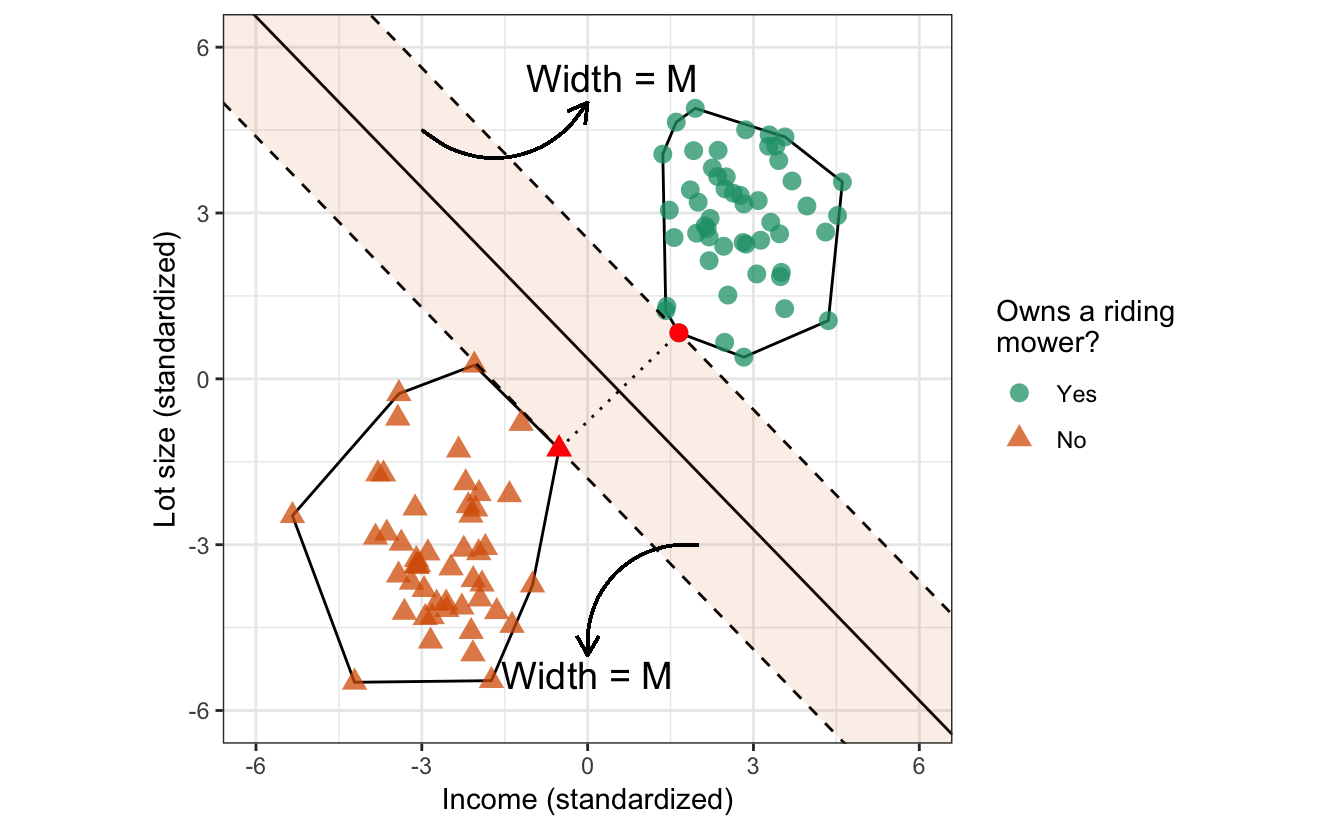
\includegraphics[width=0.8\textwidth]{figures/hmc_1}
\end{frame}

\begin{frame}{HMC Optimization Problem}
    The Hard Margin Classifier solves the following quadratic programming problem:
    \begin{block}{Optimization}
        Maximize $M$ with respect to $\beta_0, \beta_1, \dots, \beta_p.$ \\
        Subject to:
        $$\sum_{j=1}^{p} \beta_j^2 = 1$$
        $$y_i(\beta_0 + \beta_1 x_{i1} + \dots + \beta_p x_{ip}) \ge M, \quad i=1,\dots,n$$
    \end{block}
    \textit{Note: HMC allows no points on the wrong side of the margin.}
\end{frame}

\begin{frame}{The Soft Margin Classifier (SMC)}
    \begin{itemize}
        \item Hard margins are sensitive to outliers and may not generalize well.
        \item SMC allows some points to cross the margin boundaries.
        \item Introduces \textbf{slack variables} ($\xi_i$) and a \textbf{cost parameter (C)}.
        \item $C$ represents the allowable ``budget'' for total overlap.
        \item Varying $C$ makes the model robust to outliers.
    \end{itemize}
\end{frame}

\begin{frame}{The Soft Margin Classifier (Cont.)}
    \centering
    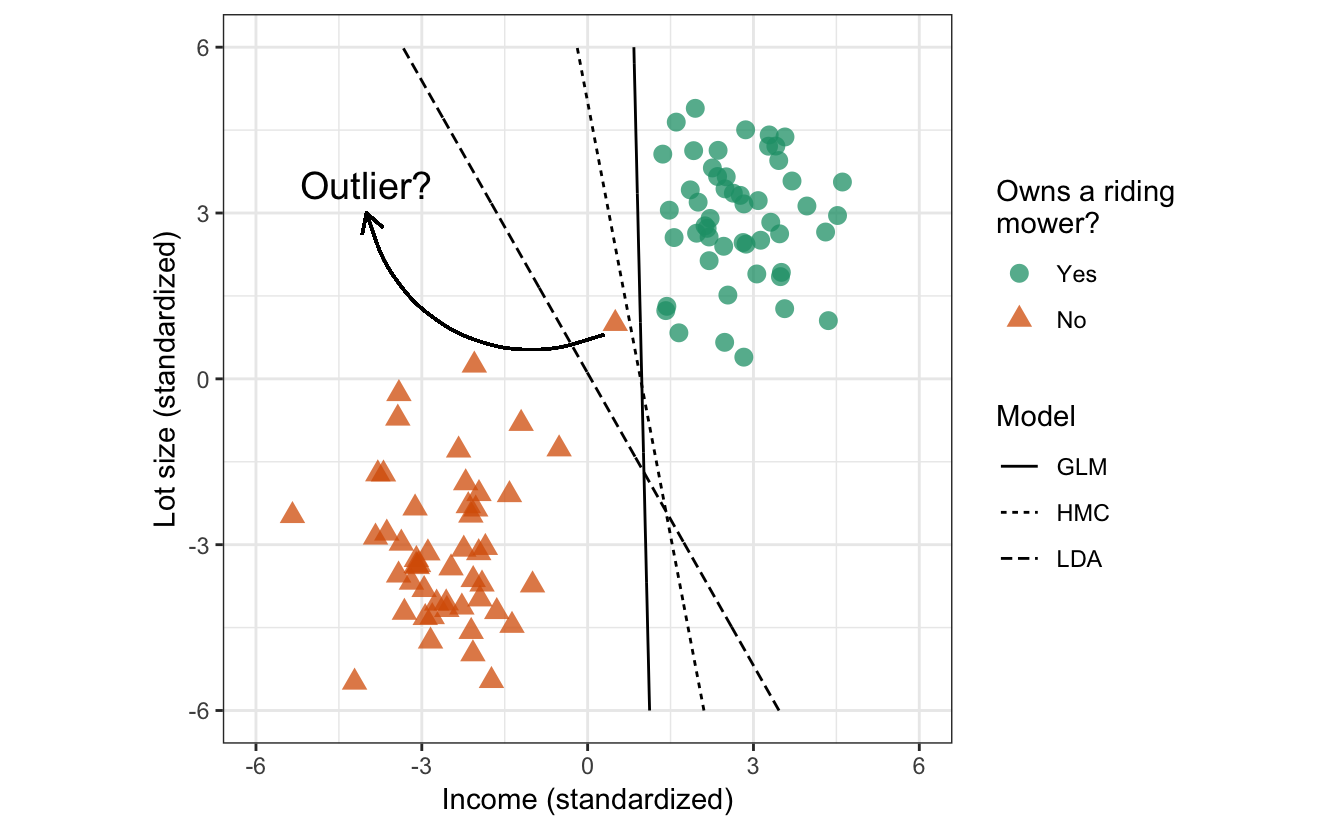
\includegraphics[width=0.8\textwidth]{figures/smc_1}
\end{frame}

\begin{frame}{The Soft Margin Classifier (Cont.)}
    \centering
    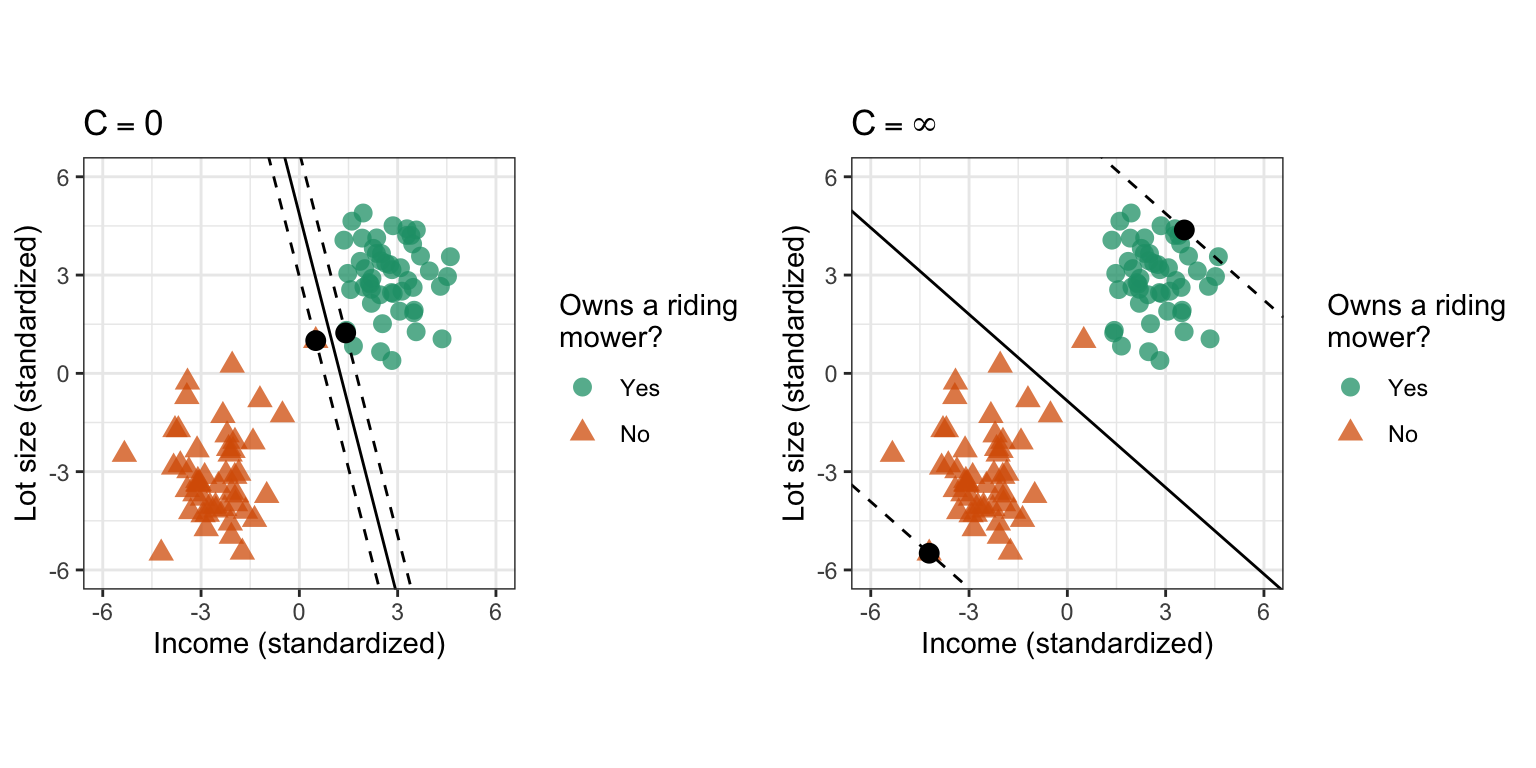
\includegraphics[width=\textwidth]{figures/smc_2}
\end{frame}

\begin{frame}{The Support Vector Machine \& Kernel Trick}
    \begin{itemize}
        \item Linear boundaries are often too restrictive for complex data.
        \item The \textbf{kernel trick} enlarges the feature space using basis functions.
        \item A hyperplane can separate classes in the \textit{enlarged} space, which becomes a \textbf{nonlinear} boundary when projected back to the original space.
        \item Example: Adding $X_3 = X_1^2 + X_2^2$ to separate nested circles.
    \end{itemize}
\end{frame}

\begin{frame}{Common Kernel Functions}
    \begin{itemize}
        \item \textbf{Polynomial:} $K(x,x') = (1 + \langle x,x' \rangle)^d$.
        \item \textbf{Radial Basis Function (RBF):} $K(x,x') = \exp(-\gamma ||x - x'||^2)$.
        \item \textbf{Hyperbolic Tangent:} $K(x,x') = \tanh(k_1 ||x - x'|| + k_2)$.
        \item The RBF kernel is extremely flexible and is usually the default starting point in practice.
    \end{itemize}
\end{frame}

\begin{frame}{Common Kernel Functions (Cont.)}
    \centering
    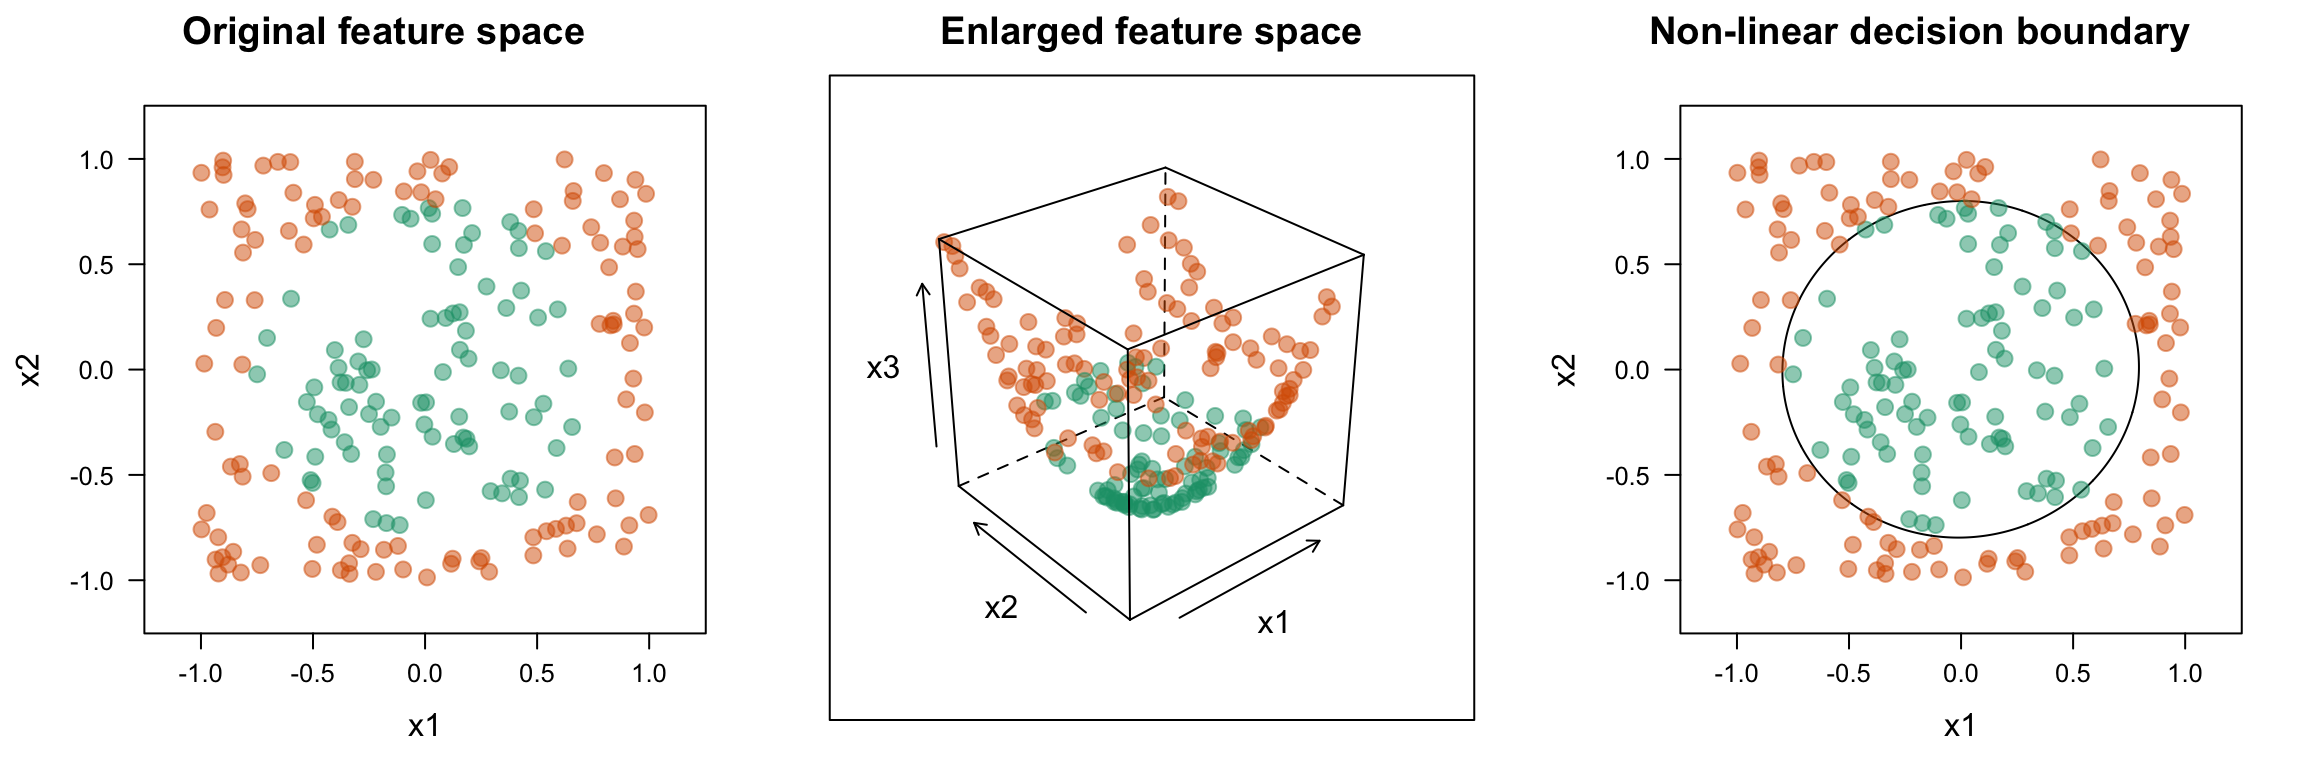
\includegraphics[width=\textwidth]{figures/circle_1}
\end{frame}

\begin{frame}{Common Kernel Functions (Cont.)}
    \centering
    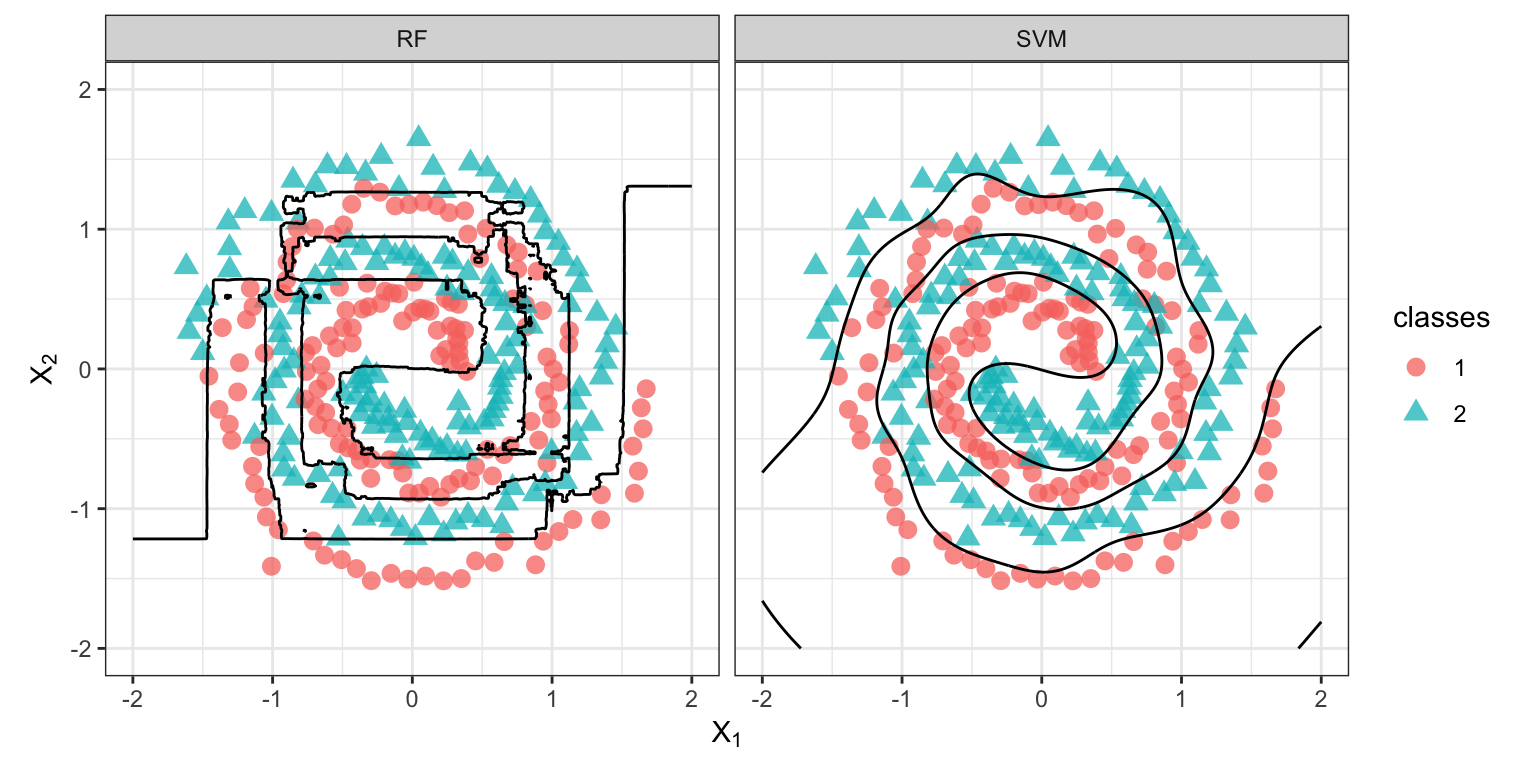
\includegraphics[width=\textwidth]{figures/spirals_1}
\end{frame}

\begin{frame}{Multinomial Classification}
    SVM is natively a binary classifier. For $>2$ classes, two strategies are used:
    \begin{itemize}
        \item \textbf{One-Versus-All (OVA):} Fit an SVM for each class against the rest. Classify based on the largest margin.
        \item \textbf{One-Versus-One (OVO):} Fit SVMs for all pairwise combinations. Classify to the class that wins the most competitions.
        \item R packages like \texttt{kernlab} handle these automatically.
    \end{itemize}
\end{frame}

\begin{frame}{Support Vector Regression (SVR)}
    \begin{itemize}
        \item SVMs extend to continuous outcomes.
        \item Uses \textbf{$\varepsilon$-insensitive loss}: residuals smaller than $\varepsilon$ have zero influence on the fit.
        \item It forms a ``margin band'' around the regression curve.
        \item SVR is more robust to outliers than Least Squares because it doesn't square the residuals.
    \end{itemize}
\end{frame}

\begin{frame}{Support Vector Regression (Cont.)}
    \centering
    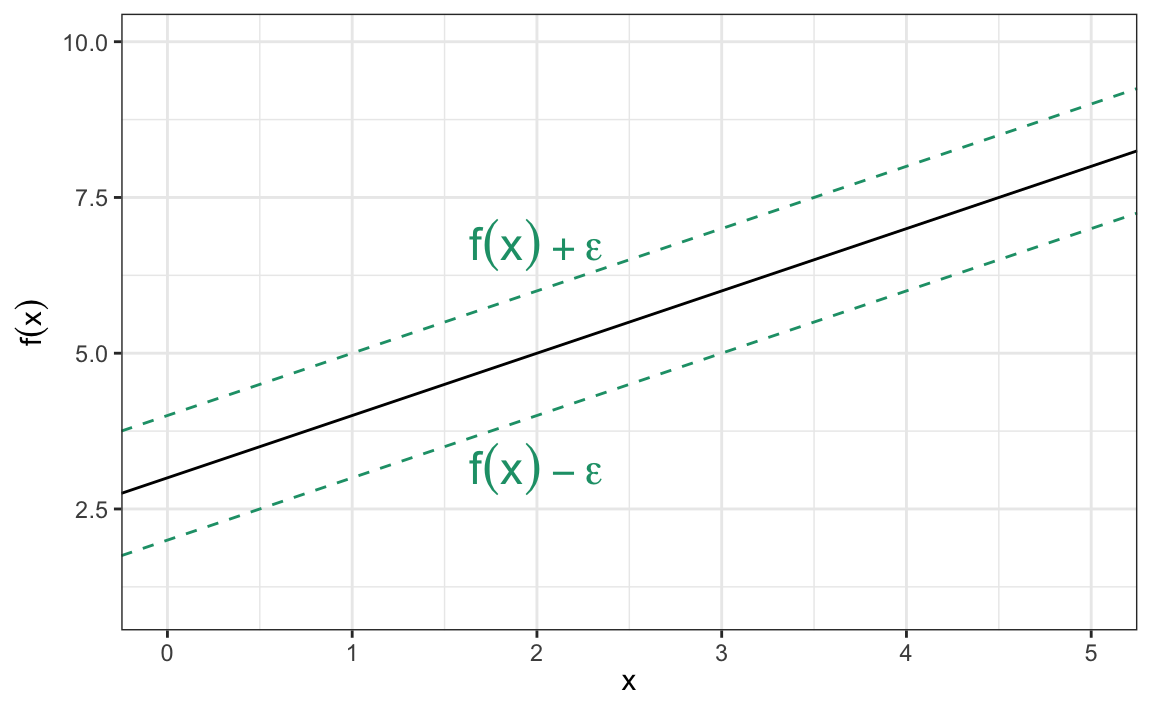
\includegraphics[width=0.8\textwidth]{figures/svr_1}
\end{frame}

\begin{frame}{Support Vector Regression (Cont.)}
    \centering
    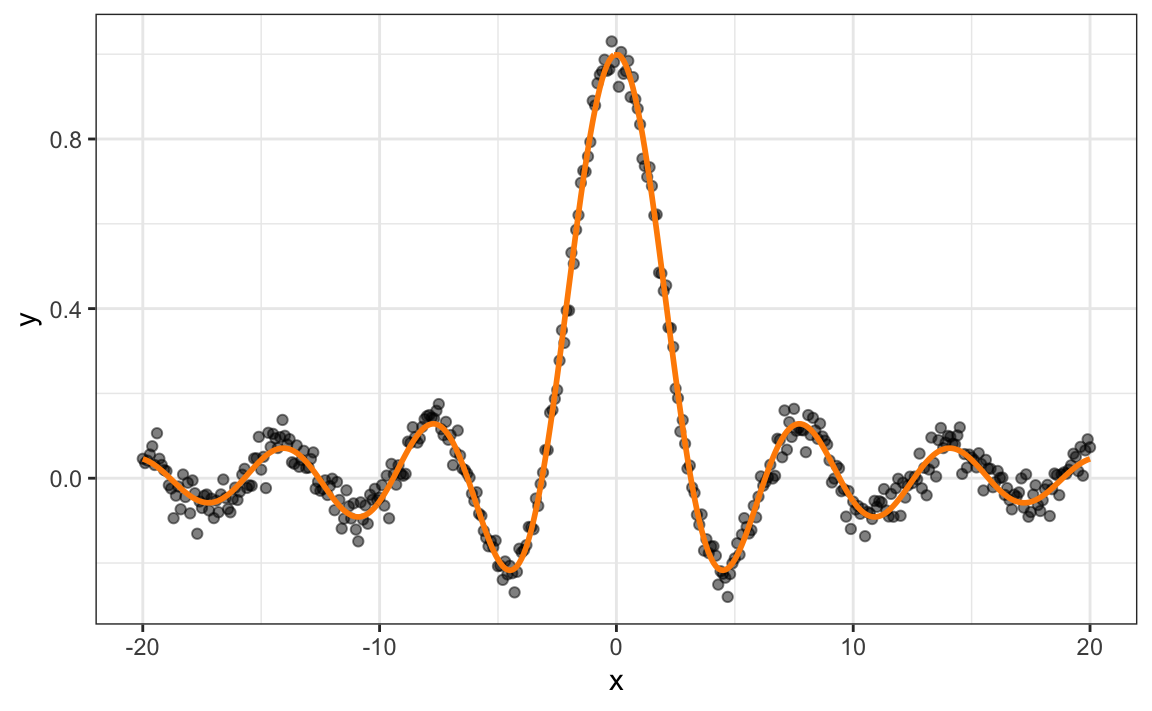
\includegraphics[width=0.9\textwidth]{figures/svr_2}
\end{frame}

\begin{frame}{Support Vector Regression (Cont.)}
    \centering
    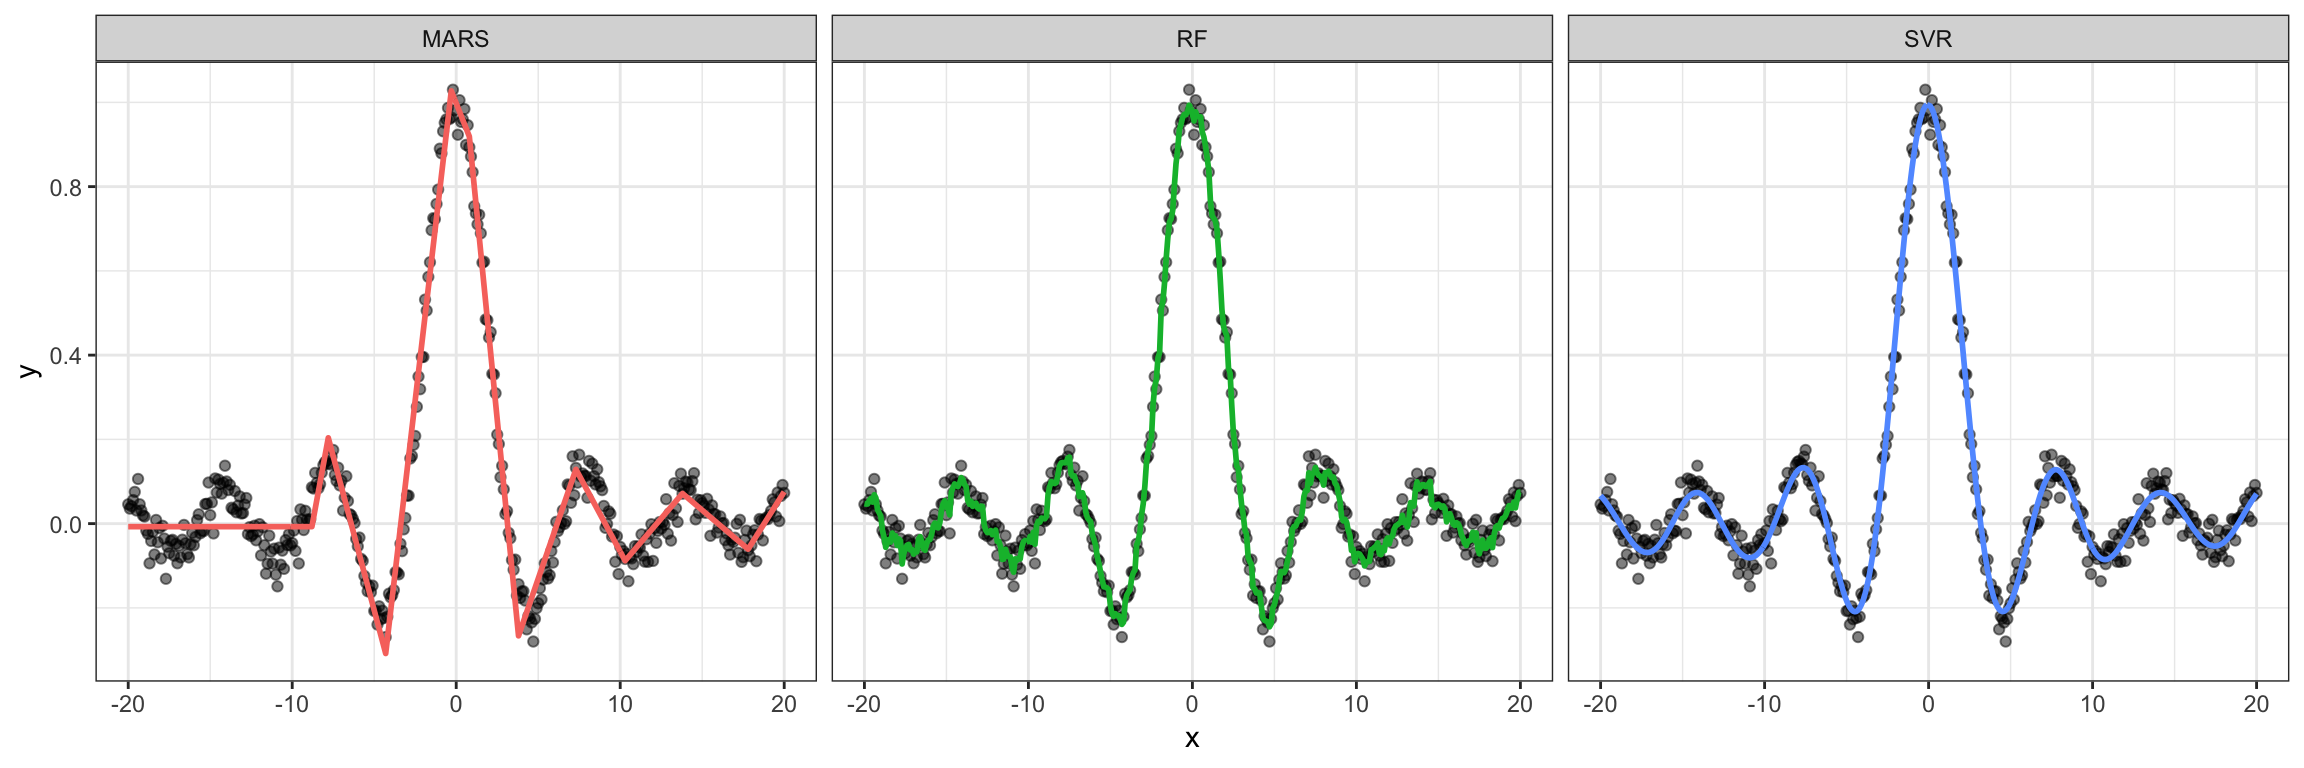
\includegraphics[width=\textwidth]{figures/svr_3}
\end{frame}

\begin{frame}{Tuning and Implementation}
    \begin{itemize}
        \item SVMs require tuning hyperparameters like \textbf{C} (cost) and \textbf{$\sigma$ / $\gamma$} (kernel parameter).
        \item In \texttt{caret}, use \texttt{train()} with \texttt{method = "svmRadial"}.
        \item The \texttt{sigest()} function in \texttt{kernlab} can provide good automated estimates for $\sigma$.
        \item Cost parameter $C$ is typically searched over an exponentially growing series (e.g., $2^{-2}, \dots, 2^8$).
    \end{itemize}
\end{frame}

\begin{frame}{Tuning and Implementation (Cont.)}
    \centering
    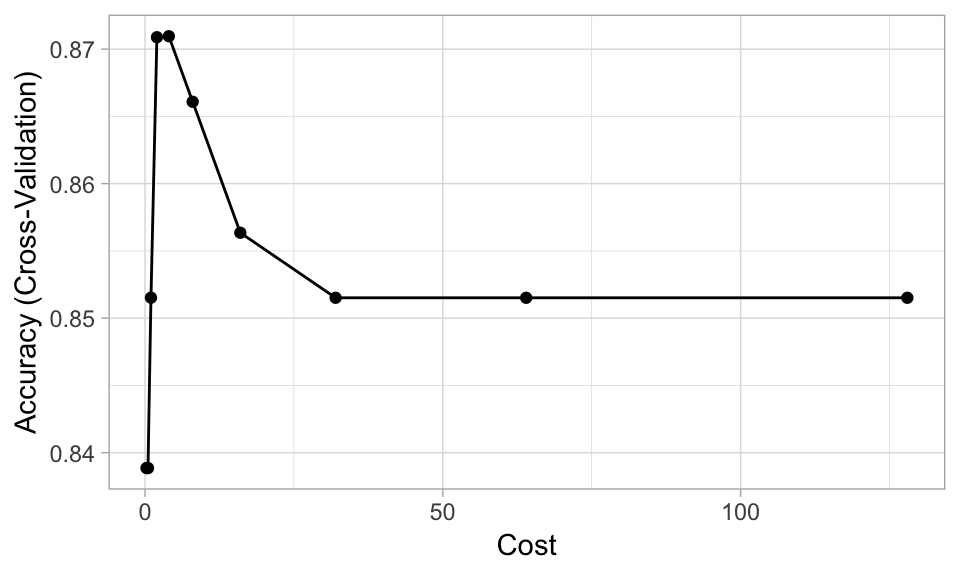
\includegraphics[width=0.8\textwidth]{figures/attrition_1}
\end{frame}

\begin{frame}{Advanced Considerations}
    \begin{itemize}
        \item \textbf{Class Imbalance:} Use \texttt{class.weights} to assign higher costs to misclassifying the minority class.
        \item \textbf{Probabilities:} SVMs don't naturally provide probabilities. Set \texttt{prob.model = TRUE} or \texttt{classProbs = TRUE} to estimate them via Platt scaling.
        \item Useful for metrics like AUC (Area Under the Curve).
    \end{itemize}
\end{frame}

\begin{frame}{Feature Interpretation}
    \begin{itemize}
        \item SVMs do not have a built-in feature importance measure.
        \item \textbf{Permutation Approach:} Use the \texttt{vip} package to measure how much a metric (like AUC) drops when a feature is shuffled.
        \item \textbf{Partial Dependence Plots (PDPs):} Use the \texttt{pdp} package to visualize the relationship between the top features and the predicted probability.
    \end{itemize}
\end{frame}

\begin{frame}{Feature Interpretation (Cont.)}
    \centering
    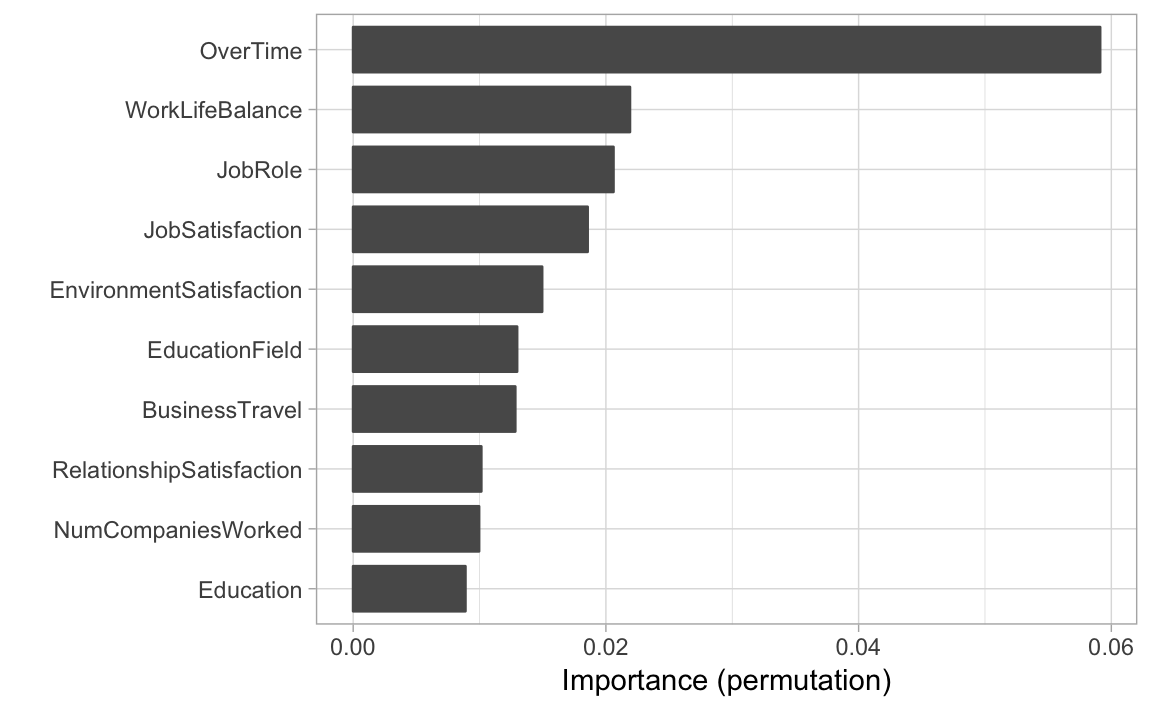
\includegraphics[width=0.8\textwidth]{figures/vip_1}
\end{frame}

\begin{frame}{The Support Vectors}
    \begin{itemize}
        \item Support vectors are the data points that lie closest to the decision boundary.
        \item These specific observations ``support'' the hyperplane; if they were moved, the boundary would shift.
        \item In an RBF or non-linear kernel, these points represent the most difficult cases to classify.
        \item Most of the training data (those far from the boundary) have no impact on the final model, making SVMs memory-efficient for prediction.
    \end{itemize}
\end{frame}

\begin{frame}{Slack Variables and the Soft Margin}
    \begin{itemize}
        \item Slack variables $\xi_i$ are introduced to allow for misclassifications in non-separable data.
        \item $\xi_i = 0$: The point is on the correct side of the margin.
        \item $0 < \xi_i \le 1$: The point is within the margin but on the correct side of the hyperplane.
        \item $\xi_i > 1$: The point is on the wrong side of the hyperplane (misclassified).
        \item The optimization goal is to maximize the margin while keeping the sum of $\xi_i$ within the budget $C$.
    \end{itemize}
\end{frame}

\begin{frame}{The Influence of the Cost Parameter $C$}
    \begin{itemize}
        \item The parameter $C$ controls the tradeoff between a ``clean'' boundary and a ``wide'' margin.
        \item \textbf{Small $C$}: Allows more margin violations. This leads to a wider margin and a simpler model (Higher Bias, Lower Variance).
        \item \textbf{Large $C$}: Penalizes violations heavily. This leads to a narrow margin that tries to classify every training point correctly (Lower Bias, Higher Variance).
        \item Finding the optimal $C$ via Cross-Validation is critical to prevent overfitting.
    \end{itemize}
\end{frame}

\begin{frame}{Tuning the RBF Kernel ($\gamma$)}
    \begin{itemize}
        \item The $\gamma$ (sigma) parameter defines how far the influence of a single training example reaches.
        \item \textbf{Low $\gamma$}: A single point has a ``far-reaching'' influence. The resulting decision boundary is smooth and less wiggly.
        \item \textbf{High $\gamma$}: Influence is localized. The boundary will stay close to individual points, potentially leading to ``islands'' around data.
        \item High $\gamma$ values risk overfitting the training data by creating a complex, irregular boundary.
    \end{itemize}
\end{frame}

\begin{frame}{Importance of Data Pre-processing}
    \begin{itemize}
        \item SVMs calculate distances between points to determine the hyperplane and margin.
        \item Because of this, SVMs are \textbf{not} scale-invariant.
        \item Features with larger ranges (e.g., ``Income'' vs. ``Years of Education'') will dominate the distance calculation.
        \item \textbf{Standardization} (centering to mean 0 and scaling to SD 1) is a mandatory step before training an SVM to ensure all features contribute equally.
    \end{itemize}
\end{frame}

\begin{frame}{Final Thoughts: Advantages and Disadvantages}
    \begin{columns}
        \begin{column}{0.5\textwidth}
            \textbf{Advantages}
            \begin{itemize}
                \item Global optimum guaranteed (convex optimization).
                \item Robust to outliers (via $C$).
                \item Extremely flexible for nonlinear data.
            \end{itemize}
        \end{column}
        \begin{column}{0.5\textwidth}
            \textbf{Disadvantages}
            \begin{itemize}
                \item Slow to train on ``tall'' data ($n \gg p$).
                \item High memory/parameter usage.
                \item Probability estimates require extra steps.
            \end{itemize}
        \end{column}
    \end{columns}
\end{frame}

\begin{frame}{Hands-On Machine Learning with R}
    \vspace{1mm}
    \centering
    
\includegraphics[height=0.75\textheight]{figures/book_cover.jpg} \\
    \vspace{1mm}
    {
        \scriptsize
        Content has been extracted from \textit{Hands-On Machine Learning with R}, by Boehmke, B. \& Greenwell, B. CRC Press. 2019.
        Visit \url{https://bradleyboehmke.github.io/HOML/}.
    }
\end{frame}

\end{document}
